\documentclass[a4paper,12pt]{article}

% Paquetes básicos
\usepackage[utf8]{inputenc}
\usepackage[T1]{fontenc}
\usepackage[spanish]{babel}
\usepackage{graphicx}
\usepackage{xcolor}
\usepackage{lipsum}
\usepackage{geometry}
\geometry{top=3cm, bottom=3cm, left=2.5cm, right=2.5cm}


% Paquetes para diseño
\usepackage{titlesec}
\usepackage{fancyhdr}
\usepackage{amsmath}
\usepackage{amssymb}
\usepackage{hyperref}
\usepackage{mathpazo}

% Paquetes para el entorno lstlisting
\usepackage{listings}
\usepackage{inconsolata}

% Paquete para fondo
\usepackage{background}

% Configuración de lstlisting
\lstset{
    inputencoding=utf8,          % Permite UTF-8
    extendedchars=true,          % Reconoce caracteres extendidos
    literate=                    % Configuración manual para tildes y símbolos
        {á}{{\'a}}1
        {é}{{\'e}}1
        {í}{{\'i}}1
        {ó}{{\'o}}1
        {ú}{{\'u}}1
        {ñ}{{\~n}}1
        {Á}{{\'A}}1
        {É}{{\'E}}1
        {Í}{{\'I}}1
        {Ó}{{\'O}}1
        {Ú}{{\'U}}1
        {Ñ}{{\~N}}1
        {¿}{{\textquestiondown}}1
        {¡}{{\textexclamdown}}1,
    basicstyle=\ttfamily,        % Fuente monoespaciada
    breaklines=true,             % Habilita salto de línea automático
    frame=single,                % Marco alrededor del código
    backgroundcolor=\color{gray!10}, % Fondo gris claro
    keywordstyle=\color{blue},   % Color para palabras clave
    commentstyle=\color{green},  % Color para comentarios
    stringstyle=\color{red}      % Color para strings
}
\lstdefinestyle{customcpp}{
    language=C++,                % Lenguaje de programación
    showspaces=false,            % No mostrar espacios
    showtabs=false,              % No mostrar tabulaciones
    tabsize=4,                   % Tamaño de tabulación
    showstringspaces=false,      % No mostrar espacios en strings
    numbers=left,                % Números de línea a la izquierda
    numberstyle=\tiny\color{gray}, % Estilo de los números de línea
    numbersep=5pt,               % Separación de los números de línea
    stepnumber=1,                % Mostrar número en cada línea
    basicstyle=\ttfamily\footnotesize, % Estilo básico del código
    keywordstyle=\bfseries\color{blue}, % Estilo de las palabras clave
    commentstyle=\itshape\color{green!50!black}, % Estilo de los comentarios
    stringstyle=\color{red},     % Estilo de los strings
    identifierstyle=\color{black}, % Estilo de los identificadores
    % procnamekeys={def,class},    % Palabras clave para nombres de funciones
    morekeywords={constexpr,nullptr,size_t}, % Más palabras clave
    emph={int,char,double,float,unsigned}, % Palabras a enfatizar
    emphstyle=\color{magenta},   % Estilo de las palabras enfatizadas
    backgroundcolor=\color{gray!10}, % Color de fondo
    frame=shadowbox,             % Marco con sombra
    rulesepcolor=\color{gray},   % Color de la línea de separación
    breakatwhitespace=false,     % No cortar en espacios en blanco
    breaklines=true,             % Cortar líneas largas
    captionpos=b,                % Posición del título (abajo)
    escapeinside={(*@}{@*)},     % Delimitadores para escapar a LaTeX
    morecomment=[l][\color{magenta}]{\#}, % Comentarios de una línea
    morecomment=[s][\color{orange}]{/*}{*/}, % Comentarios multilínea
    morestring=[b]",             % Strings entre comillas dobles
    morestring=[b]'              % Strings entre comillas simples
}


% Configuración de título
\titleformat{\section}{\normalfont\Large\bfseries}{\thesection}{1em}{}

% Información del documento
\title{
    \vspace{-2cm}
    
\includegraphics[width=0.3\textwidth]{images/etsiit.png} \\ % Cambia el logo si es necesario
    \LARGE Ingeniería Informática + ADE\\
    \large Universidad de Granada (UGR)\\[1cm]
}
\author{\textbf{Autor:} Ismael Sallami Moreno}
\date{\textbf{Asignatura:} 2º Parcial SCD}

% Configuración del fondo
\backgroundsetup{
    scale=1,
    color=black,
    opacity=0.2,
    angle=0,
    position=current page.south,
    vshift=0pt,
    hshift=0pt,
    contents={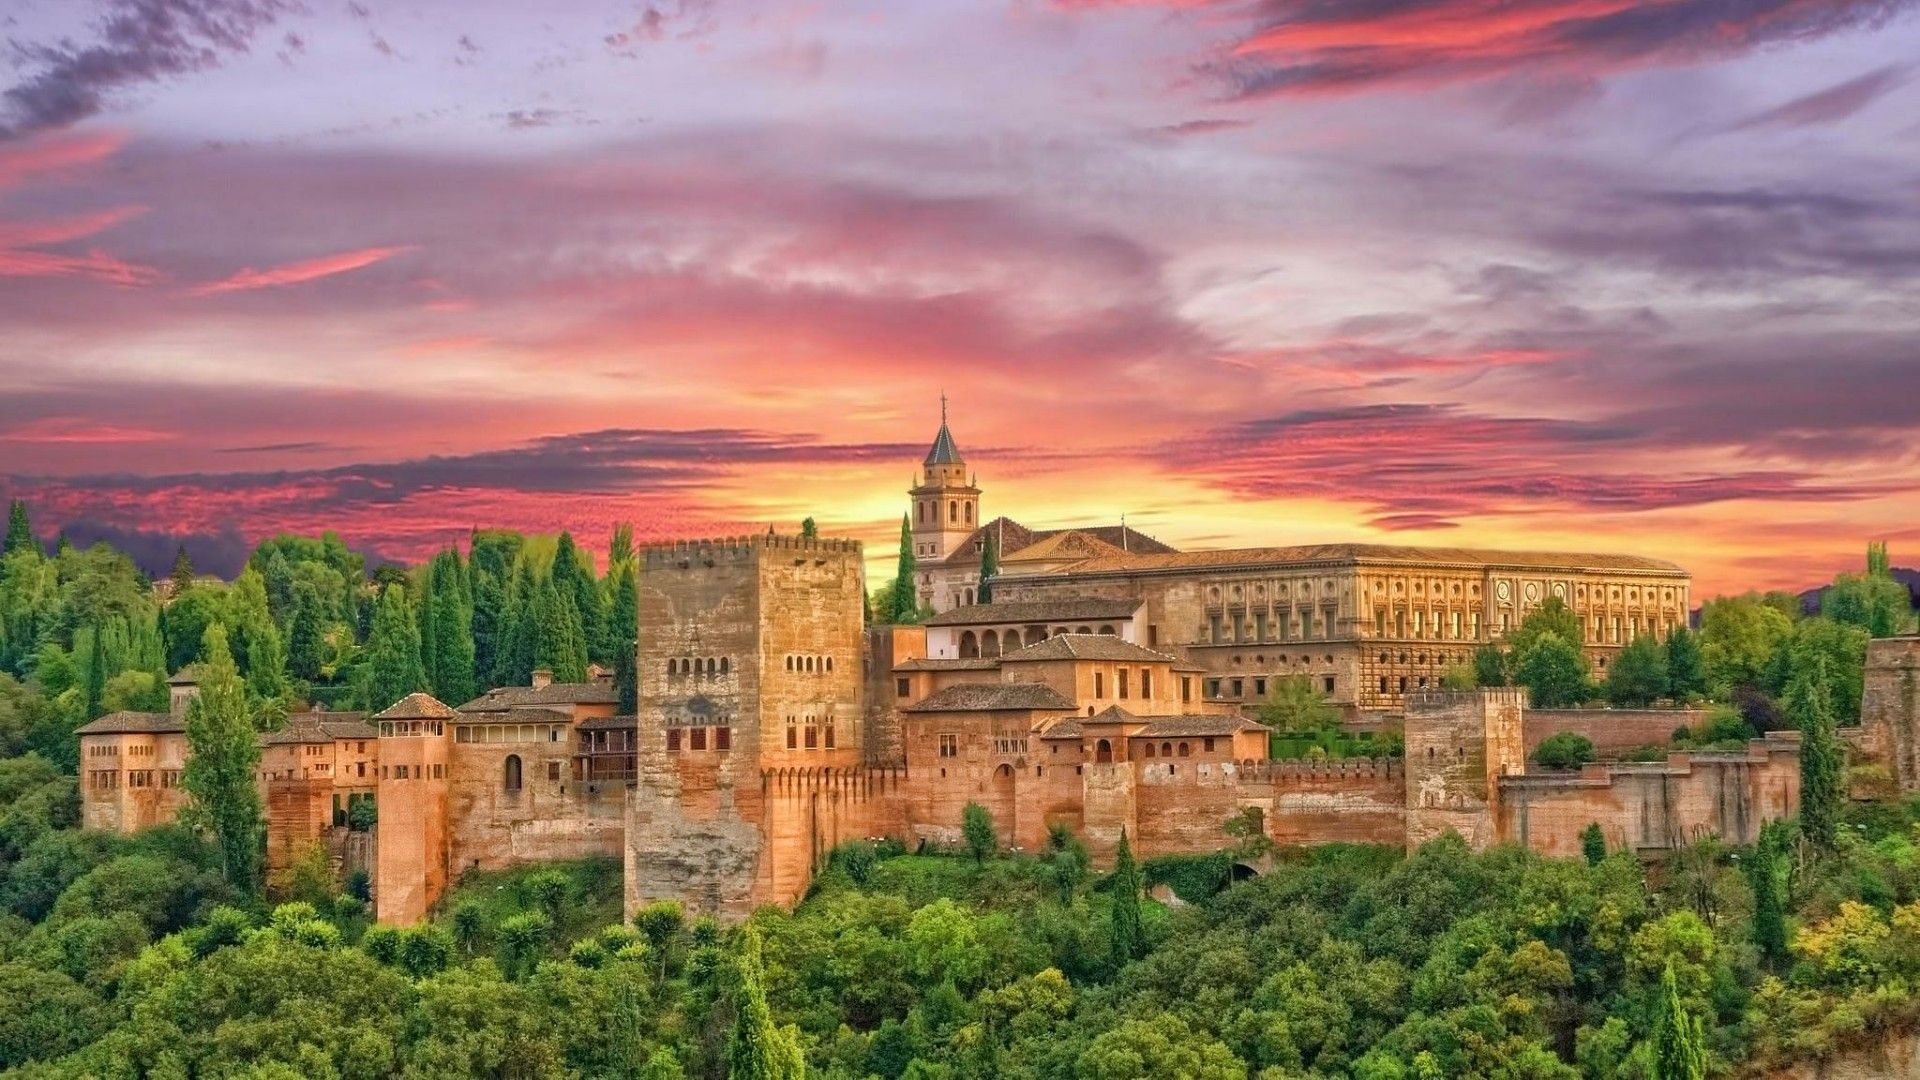
\includegraphics[width=\paperwidth,height=\paperheight,keepaspectratio]{images/granada.jpg}}
}

% Inicio del documento
\begin{document}

% Portada
\maketitle
\thispagestyle{empty}

\begin{center}
    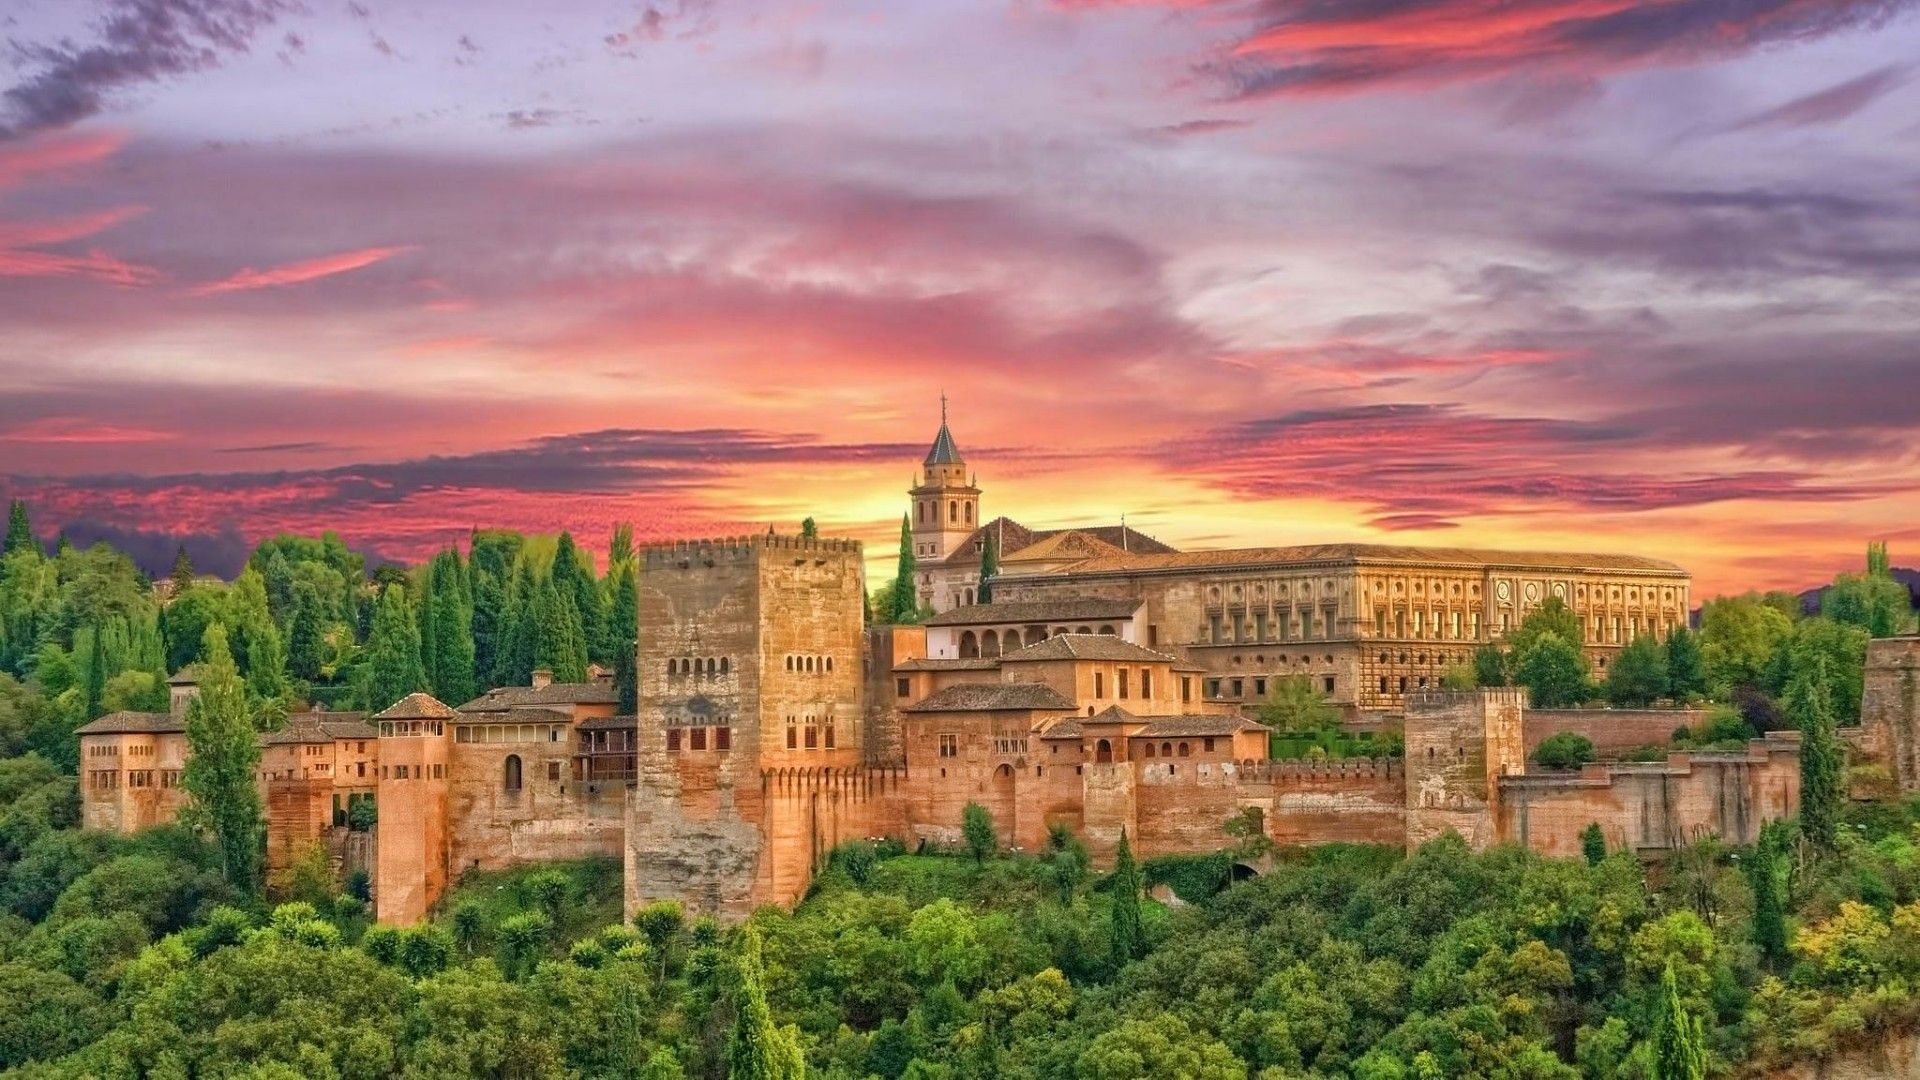
\includegraphics[width=\textwidth,height=0.4\textheight,keepaspectratio]{images/granada.jpg} \\ % Añade tu imagen de fondo
    \vfill
\end{center}

\newpage

% Índice (opcional)
\tableofcontents
\newpage

\section{Examen Carlos Ureña 2014-2015}  

\subsection{Enunciado}
\noindent
\textbf{Asignatura:} Sistemas Concurrentes y Distribuidos. \\
\textbf{Año Académico:} 2014/2015. \\
\textbf{Grado:} Doble Grado en Ingeniería Informática y ADE + Matemáticas. \\
\textbf{Descripción:} Examen correspondiente a la práctica 3 de SCD. \\
\textbf{Profesor:} Carlos Ureña. \\
\textbf{Fecha:} 12 de enero de 2015. \\


\subsubsection{Ejercicio 1. Corrección de errores (6 puntos)}

Considerar el código del archivo disponible en la subsection de plantilla de este documento o \href{https://github.com/ElblogdeIsmael/ElblogdeIsmael.github.io/blob/main/Asignaturas/Tercer%20A%C3%B1o/SCD/Examenes/SegundoParcial/ETSIIT/code/plantilla.cpp}{aquí}, que intenta plantear una solución al problema de la cena de los filósofos con camarero. Hay diversos errores en el código proporcionado que deberás solucionar:
\begin{enumerate}
    \item Intenta compilar el código proporcionado. Comprueba que hay diversos errores básicos de sintaxis que impiden que el código genere un ejecutable. Encuentra dichos errores y arréglalos hasta que el código compile correctamente. Indica en el folio del examen el número de línea y cómo debería quedar ésta una vez solventado el problema.
    \item Ejecuta el programa y observa la salida que genera. El algoritmo presenta un error en su diseño. Explica brevemente en el folio del examen por qué la salida proporcionada no es correcta.
    \item Observa el código del programa ejecutado. Encuentra y corrige el error en el diseño del algoritmo que impide que el programa muestre una salida coherente. Señala en el folio del examen en qué línea está el problema y cómo debería quedar ésta para solucionar el error.
    \item Se desea modificar el algoritmo dado del problema de los filósofos con camarero para dar servicio a 7 filósofos y 7 tenedores en lugar de a 5. También se desea cambiar el identificador de los procesos para que los filósofos sean los procesos con rank 0, 1, 2, ..., 6 y los tenedores sean los procesos 7, 8, ..., 13. Describe brevemente qué cambios debes realizar en el código proporcionado y en qué líneas.
\end{enumerate}

% \noindent
% \textbf{Solución puntos 1 y 2:} 
% En la línea 84 falta un argumento en la función \texttt{MPI\_Ssend}. No está puesto el tag del mensaje (debería ser \texttt{"segundo"}). En la línea 123 la función \texttt{MPI\_Recv} está recibiendo los dos primeros argumentos al revés: primero debe enviarse el valor y después el tamaño del envío. \\

% En cuanto al diseño, el error en la salida está en que ningún filósofo puede levantarse de la mesa cuando termina de comer. Debe haber algún fallo al enviar el mensaje al camarero para solicitar levantarse. Este se encuentra en la línea 101, en el paso del mensaje al camarero para solicitar levantarse, el tag del mensaje es el de sentarse (\texttt{TAG\_SENTARSE}), en lugar del de levantarse (\texttt{TAG\_LEVANTARSE}).

\subsubsection{Ejercicio 2. Problema de múltiples Productores-Consumidores con Paso de Mensajes (4 puntos)}

Partiendo del algoritmo desarrollado durante la Práctica 3 para resolver el problema de múltiples Productores-Consumidores usando paso de mensajes MPI, se pide realizar los siguientes cambios:
\begin{itemize}
    \item El valor que los procesos productores que envían al buffer debe ser un valor aleatorio entre 0 y 9 en lugar de uno secuencial como hasta ahora.
    \item Así mismo, el productor deberá enviar un mensaje al buffer pidiendo permiso para enviar el valor, y el buffer deberá responder al productor autorizando a enviar el mensaje antes de hacerlo (al igual que ya hace el consumidor).
\end{itemize}

Realiza los cambios necesarios para que, en el caso de que en el buffer se almacenen dos valores iguales consecutivos (independientemente del productor que los envíe), el buffer finalice.
\begin{itemize}
    \item Antes de finalizar deberá avisar a todos los productores y consumidores para que estos finalicen enviando un valor especial en los mensajes de autorización (por ejemplo, un valor negativo). Sólo cuando todos los procesos hayan finalizado el buffer terminará.
    \item Implementa esta condición de forma que cuando cualquier proceso vaya a finalizar, imprima un mensaje en pantalla informando de ello.
\end{itemize}

\subsubsection{Plantilla}

\lstinputlisting[style=customcpp]{code/ExamenCarlos/plantilla.cpp}
% iconv -f ISO-8859-1 -t UTF-8 plantilla.cpp -o plantilla_utf8.cpp


\subsection{Solución Carlos Ureña 2014-2015}

\subsubsection*{Ejercicio 1}
\begin{itemize}
    \item Errores:
    \begin{itemize}
        \item En la línea 84 falta un argumento en la función \texttt{MPI\_Ssend}. No está puesto el tag del mensaje (debería ser \texttt{"segundo"}).
        \item En la línea 124 que los dos primeros argumentos están al revés.
    \end{itemize}
    \item Error en el diseño: podemos ver que tras la ejecución del programa, los filósofos no se levantan de la mesa. El error se encuentra en la línea 101, en el paso del mensaje al camarero para solicitar levantarse, el tag del mensaje es el de sentarse (\texttt{TAG\_SENTARSE}), en lugar del de levantarse (\texttt{TAG\_LEVANTARSE}).
    \item Último apartado: 
    \begin{itemize}
        \item para dar servicio a 7 filósofos y 7 tenedores, se deben cambiar las constantes \texttt{NUM\_FILOSOFOS} en la línea 7.
        \item para ello debemos de cambiar la línea 54 poniendo que el rank debe de ser menor al número de filósofos.
        \item además, debemos de cambiar la asignación de los tenedores en la línea 68 y 69, debido a que la presente no es coherente ni consistente desembocando en un error en el que varios filósofos quieren coger el mismo tenedor.
    \end{itemize}
\end{itemize}
\lstinputlisting[style=customcpp]{code/ExamenCarlos/ejercicio.cpp}
La solución en código se encuentra \href{https://github.com/ElblogdeIsmael/ElblogdeIsmael.github.io/blob/main/Asignaturas/Tercer%20A%C3%B1o/SCD/Examenes/SegundoParcial/ETSIIT/code/ejercicio.cpp}{aqui}.

\subsubsection*{Ejercicio 2}

En la resolución de este ejercicio usamos esta \href{https://github.com/ElblogdeIsmael/ElblogdeIsmael.github.io/blob/main/Asignaturas/Tercer%20A%C3%B1o/SCD/Examenes/SegundoParcial/ETSIIT/code/prodcons2-muPlantilla.cpp}{(plantilla)}(pincha en plantilla para acceder a ella).

\begin{itemize}
    \item Hemos añadido en la línea 58 en la función de producir valor esta línea \textbf{int valor = aleatorio<0, 9>();} para que produzca el valor aleatorio.
    \item En la función del productor debemos añadir \textbf{MPI\_Ssend(\&peticion, 1, MPI\_INT, n\_p, etiq\_productor, MPI\_COMM\_WORLD);} para que el productor pida permiso para enviar el valor y añadimos en el \textbf{switch} que cuando sea el caso del productor reciba la petición de aviso: \textbf{MPI\_Recv(\&peticion\_productor, 1, MPI\_INT, MPI\_ANY\_SOURCE, etiq\_productor, MPI\_COMM\_WORLD, \&estado);}
\end{itemize}


Para la solución del apartado 2.2 revisa este código donde los comentarios \textbf{apartado2.2} reflejan los cambios que se han realizado.

\lstinputlisting[style=customcpp]{code/ExamenCarlos/prodcons2-mu.cpp}
Pincha \href{https://github.com/ElblogdeIsmael/ElblogdeIsmael.github.io/blob/main/Asignaturas/Tercer%20A%C3%B1o/SCD/Examenes/SegundoParcial/ETSIIT/code/prodcons2-mu.cpp}{aqui} para acceder al fichero.


\section{Examen de Mario Bros con Yoshi como NPC}

\subsection{Enunciado}

Se pide resolver el siguiente ejercicio utilizando directivas MPI vistas en clase. El juego consiste en comer tantas tartas como sea posible. El que más kg de tartas haya comido, gana. Contaremos con las siguientes restricciones:

\begin{itemize}
    \item Habrá solamente dos jugadores, Mario y Peach.
    \item Habrá un NPC, Yoshi, que será el árbitro.
    \item El proceso Yoshi se encargará:
    \begin{itemize}
        \item Por un lado, de proveer tartas a cada equipo. Repondrá un máximo de x veces.
        \begin{itemize}
            \item Cada vez que repone, decide si provee de 1 o 2 tartas a la vez. Creará un vector con 1 o 2 elementos.
            \item Cada tarta tendrá un peso asociado que será también aleatorio entre 1 y 10 kg. Un vector [1,10] indicará el peso mínimo y máximo de las tartas.
            \item Mostrará cuántas tartas va a reponer y a qué equipo.
        \end{itemize}
        \item Por otro lado, recibirá la suma de los kg que cada equipo se ha comido en cada tanda. Para cada tanda servida:
        \begin{itemize}
            \item Comparará quién ha comido más kg de tarta en dicha tanda.
            \item Sumará 1 punto al equipo que más kg haya comido.
        \end{itemize}
        \item Finalmente, comparará los puntos de ambos equipos y proclamará vencedor al que más kg de tarta comió.
    \end{itemize}
    \item Los procesos Mario y Peach realizarán las siguientes operaciones:
    \begin{itemize}
        \item Recibirán las tartas que se van a comer.
        \item Mostrarán las tartas que han recibido y sus pesos.
        \item Sumarán el peso de cada tarta y aleatoriamente se comerán una porción.
        \item La cantidad que se han comido se la notificarán a Yoshi.
    \end{itemize}
    \item Mientras haya envíos que hacer, se han de poder realizar, evitando que haya ningún tipo de bloqueo. Es decir, Yoshi podrá reponer tartas sin tener que sufrir ningún tipo de bloqueo por otras operaciones (a excepción de retrasos aleatorios).
    \item Se han de incluir retrasos aleatorios.
\end{itemize}
%enunciado

\subsection{Solución}
\lstinputlisting[style=customcpp]{code/ExamenYoshi/Solucion.cpp}

\section{Examen de Consumidores (valores pares e impares)}

\subsection{Enunciado}
%enunciado
Se pide modificar la solución al problema de múltiples productores y consumidores realizada en clase utilizando directivas MPI, de forma que:

\begin{itemize}
    \item El número de productores sea 3 (y que pueda variar fácilmente).
    \item El número de consumidores sea 2, de forma que:
    \begin{itemize}
        \item Habrá un consumidor que solo pueda consumir los valores pares.
        \item El otro consumidor solo podrá consumir los valores impares.
    \end{itemize}
\end{itemize}

\subsection{Solución}
\subsubsection{Partimos de la plantilla}
\lstinputlisting[style=customcpp]{code/ExamenConsumidoresParesImpares/prodcons2-mu.cpp}
\subsubsection{Solución}
\lstinputlisting[style=customcpp]{code/ExamenConsumidoresParesImpares/prodcons2-muSolucion.cpp}

\section{Examen de modificar camarero y filósofos}
\subsection{Enunciado}

El archivo plantilla proporcionado contiene una solución básica al problema de los filósofos con camarero. En esta solución, el camarero se encarga de controlar el acceso a la mesa, permitiendo que se sienten a la mesa un máximo de 4 filósofos. Hay 5 filósofos.

Modificar este archivo como sigue:

\begin{itemize}
    \item El filósofo 4, cuyo rango es 8, tendrá un comportamiento algo diferente del resto. El filósofo 4 no pide ni suelta ningún tenedor ya que come con las manos. No obstante, este filósofo sí debe pedir permiso para sentarse y levantarse al camarero.
    \item Como el filósofo 4 no puede comer si no se siente muy acompañado, el camarero solo permite que se siente cuando hay 4 filósofos sentados en ella.
    \item El camarero además no permite levantarse a ninguno de ellos mientras está comiendo el filósofo 4, para que se sienta acompañado.
    \item Como ahora ya no hay interbloqueo, podría haber 5 sentados en la mesa. Han de usarse unas etiquetas especiales para el filósofo 4.
\end{itemize}

El camarero deberá, en un bucle infinito:

\begin{itemize}
    \item Paso 1 (Usar Iprobe)
    \begin{itemize}
        \item IF (hay menos de 4 sentados)
        \begin{itemize}
            \item Sondeo en un bucle de las peticiones de sentarse o levantarse de cualquier filósofo distinto al 4, hasta detectar una.
            \item Recibe el primer mensaje detectado.
        \end{itemize}
        \item ELSE IF (hay 4)
        \begin{itemize}
            \item Sondeo en un bucle de las peticiones de levantarse de los filósofos distintos al 4 y de sentarse del 4, hasta detectar una.
            \item Recibe el primer mensaje detectado.
        \end{itemize}
        \item ELSE
        \begin{itemize}
            \item Recibe la petición de levantarse del filósofo 4.
        \end{itemize}
    \end{itemize}
    \item Paso 2
    \begin{itemize}
        \item Actualiza el número de sentados (en función de la etiqueta recibida).
    \end{itemize}
\end{itemize}
%enunciado

\subsection{Solución}
\subsubsection{Partimos de la plantilla}
\lstinputlisting[style=customcpp]{code/ExamenCamarero/plantilla.cpp}
\subsubsection{Solución}
\lstinputlisting[style=customcpp]{code/ExamenCamarero/Solucion.cpp}

\section{Examen Realizado del grupo A3 de este curso}
\subsection{Enunciado}
Se iba detallando los pasos que se debía de hacer, en este caso en la función del proceso encargado se debía de consultar el valor de cajas disponibles, en mi caso lo hice así por simplicidad.
\subsection{Solución}
\lstinputlisting[style=customcpp]{code/examen3.cpp}

\section{Materiales}
Los materiales se encuentran en mi página web (pincha \href{https://github.com/ElblogdeIsmael/ElblogdeIsmael.github.io/tree/main/Asignaturas/Tercer%20A%C3%B1o/SCD/Examenes/SegundoParcial/ETSIIT/code}{aqui}.)

\end{document}
